\chapter{Zakończenie}
\label{chapt:Zakonczenie}

% ─────────────────────────────────────────────────────────────────────────────
\section{Podsumowanie zrealizowanych prac}
\label{sec:summary}
% ─────────────────────────────────────────────────────────────────────────────

Celem projektu VT-LAN było stworzenie aplikacji desktopowej umożliwiającej
komunikację głosową i tekstową w obrębie sieci lokalnej (LAN), bez
konieczności korzystania z zewnętrznych serwerów pośredniczących. Projekt
został zrealizowany zgodnie z założeniami zaproponowanymi na etapie
planowania.

W toku prac zespół zaimplementował i zintegrował następujące komponenty:

\begin{itemize}
    \item \textbf{Infrastruktura sieciowa (backend)} -- architektura
    klient-serwer w modelu \textit{listen server}, oparta na bibliotece
    GameNetworkingSockets (GNS). Obejmuje zarządzanie pokojami i sesjami
    użytkowników, mechanizm RPC do komunikacji sterującej oraz podział ruchu
    na niezawodny kanał danych i bezgwarancyjny kanał głosowy
    (rozdział~\ref{chapt:Backend}).

    \item \textbf{Transmisja głosowa} -- przechwytywanie audio przez SDL3,
    kompresja kodekiem Opus (32\,kbps VBR, tryb VoIP, ramki 20\,ms),
    detekcja aktywności mowy (VAD) oparta na RMS z mechanizmem
    \textit{grace period}, kolejkowanie pakietów z obsługą utraty pakietów
    przez PLC dekodera Opus.

    \item \textbf{Komunikacja tekstowa i przesyłanie plików} -- czat
    tekstowy realizowany przez RPC \texttt{ChatBroadcast}, transfer plików
    z mechanizmem segmentacji i rate-limitingu zapobiegającym przepełnieniu
    buforów sieciowych, obsługa przeciągania plików na okno aplikacji
    (\textit{drag and drop}).

    \item \textbf{Bezpieczeństwo transmisji} -- wbudowane szyfrowanie
    AES-256-GCM z wymianą kluczy X25519, zapewniające poufność, integralność
    i ochronę przed atakami powtórzeniowymi. Opcjonalne hasło pokoju
    ograniczające dostęp do sesji.

    \item \textbf{Interfejs użytkownika} -- aplikacja desktopowa
    zrealizowana w Dear ImGui renderowanym przez SDL3. Widoki:
    ekran startowy, formularz tworzenia pokoju, formularz dołączania
    do pokoju, ekran zaproszenia oraz główny ekran pokoju rozmów
    z listą uczestników, czatem i panelem audio
    (rozdział~\ref{ch:interfejs_uzytkownika}).

    \item \textbf{Diagnostyka i profilowanie} -- narzędzia monitorowania
    zużycia CPU i RAM, analiza ruchu sieciowego przy użyciu Wireshark,
    testy wydajnościowe modułu audio (latencja, jitter, utrata pakietów)
    oraz czatu tekstowego (rozdział~\ref{ch:profilowanie_debugging}).
\end{itemize}

Gotowe repozytorium projektu wraz z kodem źródłowym i wersjami wydaniowymi
dostępne jest publicznie pod adresem:\\[6pt]
\url{https://github.com/Panogrodek/VT-LAN}

% ─────────────────────────────────────────────────────────────────────────────
\section{Podział prac w zespole}
\label{sec:team}
% ─────────────────────────────────────────────────────────────────────────────

Projekt realizowany był przez czteroosobowy zespół. Poniżej przedstawiono
zakres zadań każdego z członków.

\subsection*{Paweł Lipczyk -- Backend, infrastruktura sieciowa}

Odpowiedzialny za architekturę sieciową aplikacji -- model klient-serwer
w sieci LAN. Implementacja protokołów transmisji danych głosowych (UDP
z kodekiem Opus) i tekstowych (GNS reliable). Zarządzanie pokojami
i sesjami użytkowników. Integracja progu głośności (VAD --
\textit{Voice Activity Detection}) jako filtra przed transmisją audio.

\subsection*{Kacper Parys -- Bezpieczeństwo systemu, szyfrowanie}

Odpowiedzialny za dobór i implementację protokołu szyfrowania transmisji
głosowej i tekstowej w sieci LAN. Zapewnienie, że żadne dane użytkownika
nie opuszczają sieci lokalnej. Analiza potencjalnych wektorów ataku
w środowisku LAN oraz weryfikacja skuteczności zastosowanych zabezpieczeń.

\subsection*{Michał Gierszon -- Diagnostyka, profilowanie, QA}

Odpowiedzialny za dobór i integrację narzędzi profilujących w celu
monitorowania zużycia CPU, RAM oraz przepustowości sieci. Opracowanie
testów wydajnościowych dla modułu audio (utrata pakietów, latencja,
jitter) oraz czatu tekstowego. Dokumentowanie wykrytych błędów
i weryfikacja poprawek.

\subsection*{Konrad Gałka -- Frontend, UI/UX, dokumentacja}

Odpowiedzialny za projekt i implementację interfejsu użytkownika --
widok listy pokojów, panel czatu, moduł głosowy oraz dbałość o spójność
wizualną i intuicyjność obsługi, szczególnie w kontekście użycia
na wykładach. Sporządzanie dokumentacji technicznej projektu, raportów
postępu oraz przygotowanie materiałów na prezentację końcową.

% ─────────────────────────────────────────────────────────────────────────────
\section{Elementy niezrealizowane}
\label{sec:not_implemented}
% ─────────────────────────────────────────────────────────────────────────────

W pierwotnym dokumencie projektowym część funkcjonalności opisana była jako
cele szczegółowe lub ewentualne rozszerzenia. Poniżej przedstawiono
zestawienie elementów, które nie znalazły się w końcowej wersji
aplikacji, wraz z uzasadnieniem.

\subsection*{Dedykowany system anonimowych pytań}

Propozycja projektowa zakładała implementację systemu umożliwiającego
studentom anonimowe zadawanie pytań z mechanizmem grupowania podobnych
pytań oraz głosowaniem „+1". Funkcjonalność ta nie została zaimplementowana
jako odrębny moduł, ponieważ aplikacja oferuje równoważne rozwiązanie
bez dodatkowego nakładu implementacyjnego: użytkownik przy dołączaniu
do pokoju wpisuje dowolne imię i nazwisko, co pozwala na pełną anonimowość
przez podanie pseudonimu. Rozbudowany system kategoryzacji pytań
i rankingowania wymagałby implementacji algorytmów grupowania tekstu
(np. z użyciem miar podobieństwa lub prostych technik NLP), co wykraczało
poza zakres czasowy projektu i nie było niezbędne do realizacji głównych
celów -- komunikacji głosowej i tekstowej.

\subsection*{Udostępnianie ekranu i prezentacja materiałów}

Propozycja projektowa wskazywała udostępnianie ekranu lub formę
prezentacji jako \textbf{ewentualne rozszerzenie} - uwarunkowane
uprzednim ukończeniem głównych funkcjonalności. Ze względu na ograniczenia
czasowe rozszerzenie to nie zostało zrealizowane. Implementacja
przechwytywania i transmisji strumienia wideo wymagałaby dodatkowej
warstwy kodowania (np. H.264/H.265) oraz znacząco wyższej przepustowości,
co stanowiłoby odrębny zakres pracy.

% ─────────────────────────────────────────────────────────────────────────────
\section{Instrukcja obsługi aplikacji}
\label{sec:manual}
% ─────────────────────────────────────────────────────────────────────────────

Poniższa sekcja opisuje sposób pobrania, instalacji i obsługi aplikacji
VT-LAN. Pełna, aktualizowana instrukcja dostępna jest w pliku
\texttt{README.md} w repozytorium projektu pod adresem
\url{https://github.com/Panogrodek/VT-LAN}.

\subsection*{Pobieranie i instalacja}

\textbf{Krok 1 -- Pobierz aplikację.}
Należy przejść do zakładki \textbf{Releases} na stronie projektu i pobrać
najnowszą wersję aplikacji (plik \texttt{.zip}).

\textbf{Krok 2 -- Wypakuj archiwum.}
Po pobraniu pliku \texttt{.zip}:
\begin{enumerate}
    \item Kliknij prawym przyciskiem myszy na pobrany plik.
    \item Wybierz \textbf{„Wyodrębnij wszystko..."}.
    \item Wskaż folder docelowy.
    \item Otwórz wypakowany folder i uruchom plik \textbf{\texttt{VT-LAN.exe}}.
\end{enumerate}

\begin{quote}
\textbf{Uwaga:} Aplikacji nie należy uruchamiać bezpośrednio z archiwum
ZIP -- wymagane jest wcześniejsze wypakowanie zawartości.
\end{quote}

\subsection*{Pierwsze uruchomienie}

Po uruchomieniu aplikacji wyświetlany jest ekran startowy (rysunek~\ref{fig:repo_start}).
Na tym ekranie dostępne są dwie opcje:

\begin{figure}[H]
    \centering
    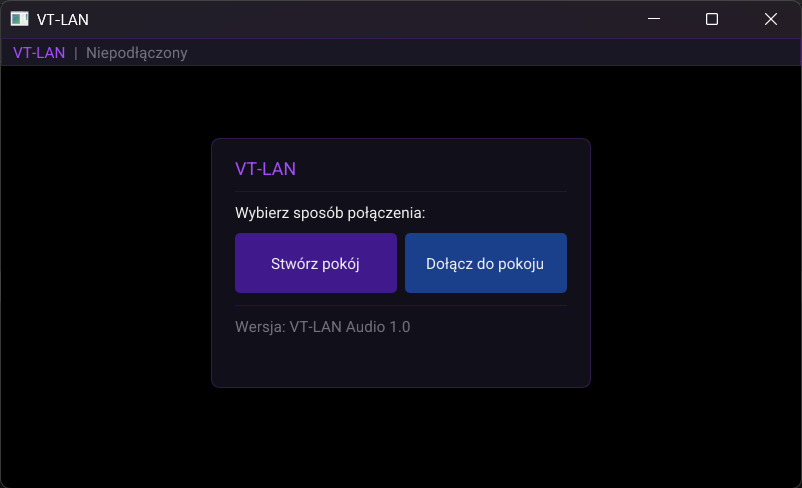
\includegraphics[width=0.70\textwidth]{figures/repo/start.png}
    \caption{Ekran startowy aplikacji VT-LAN (praca własna)}
    \label{fig:repo_start}
\end{figure}

\begin{itemize}
    \item \textbf{Utwórz pokój} -- pozwala uruchomić sesję jako host
    i oczekiwać na połączenia od innych uczestników.
    \item \textbf{Dołącz do pokoju} -- umożliwia przyłączenie się
    do istniejącej sesji utworzonej przez innego użytkownika.
\end{itemize}

\begin{quote}
\textbf{Informacja:} Dane takie jak imię i nazwisko są przechowywane
lokalnie. Przy kolejnym uruchomieniu aplikacji pola te zostaną wypełnione
automatycznie.
\end{quote}

\subsection*{Tworzenie pokoju (Host)}

Aby zaprosić innych uczestników do rozmowy, należy wybrać opcję
\textbf{„Utwórz pokój"}. Formularz tworzenia pokoju przedstawiono
na rysunku~\ref{fig:repo_host}. Zawiera on następujące pola:

\begin{figure}[H]
    \centering
    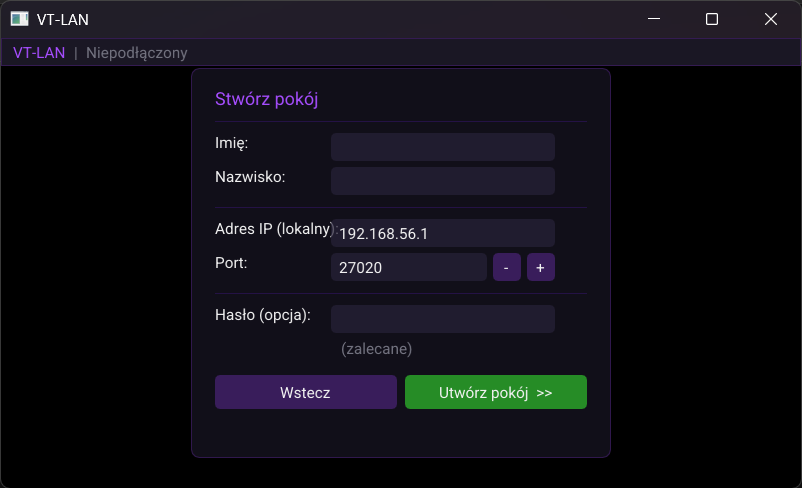
\includegraphics[width=0.70\textwidth]{figures/repo/host.png}
    \caption{Formularz tworzenia pokoju (Host) (praca własna)}
    \label{fig:repo_host}
\end{figure}

\begin{table}[H]
    \centering
    \caption{Pola formularza tworzenia pokoju}
    \begin{tabularx}{\textwidth}{|l|X|}
        \hline
        \textbf{Pole} & \textbf{Opis} \\
        \hline
        Imię & Imię widoczne dla pozostałych uczestników \\
        \hline
        Nazwisko & Nazwisko widoczne dla pozostałych uczestników \\
        \hline
        Port & Numer portu używanego do połączenia. Domyślna wartość
               (27020) nie wymaga zmiany w typowych warunkach \\
        \hline
        Hasło \textit{(opcjonalne)} & Ogranicza dostęp do pokoju --
               tylko osoby znające hasło będą mogły dołączyć.
               Pozostawienie pola pustego oznacza brak zabezpieczenia hasłem \\
        \hline
    \end{tabularx}
    \label{tab:host_form}
\end{table}

Adres IP pobierany jest automatycznie na podstawie adresu urządzenia
w sieci lokalnej. Po wypełnieniu formularza należy kliknąć
\textbf{„Utwórz"}, aby uruchomić pokój.

\subsection*{Dołączanie do pokoju (Klient)}

Aby dołączyć do istniejącej sesji, należy wybrać opcję
\textbf{„Dołącz do pokoju"}. Formularz dołączania do pokoju
przedstawiono na rysunku~\ref{fig:repo_client}. Zawiera on następujące pola:

\begin{figure}[H]
    \centering
    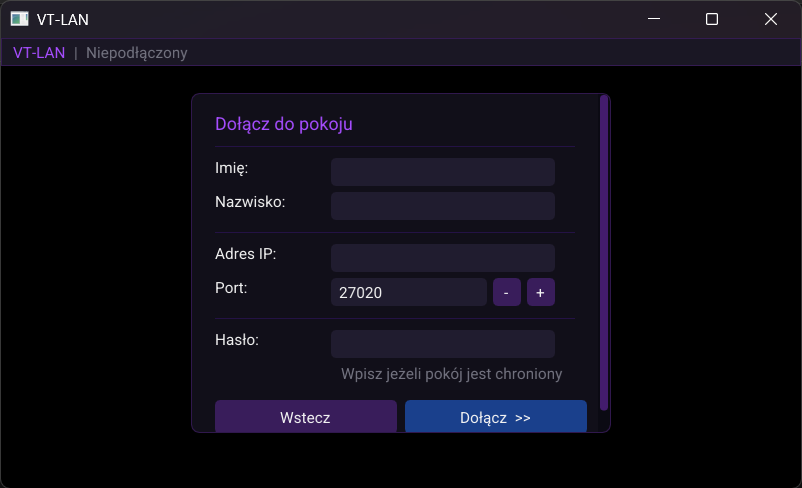
\includegraphics[width=0.70\textwidth]{figures/repo/client.png}
    \caption{Formularz dołączania do pokoju (Klient) (praca własna)}
    \label{fig:repo_client}
\end{figure}

\begin{table}[H]
    \centering
    \caption{Pola formularza dołączania do pokoju}
    \begin{tabularx}{\textwidth}{|l|X|}
        \hline
        \textbf{Pole} & \textbf{Opis} \\
        \hline
        Imię & Imię widoczne dla pozostałych uczestników \\
        \hline
        Nazwisko & Nazwisko widoczne dla pozostałych uczestników \\
        \hline
        Adres IP hosta & Adres IP urządzenia hosta -- dostępny
                         w otrzymanym zaproszeniu \\
        \hline
        Port & Numer portu podany przez hosta \\
        \hline
        Hasło \textit{(jeśli wymagane)} & Wymagane wyłącznie w przypadku,
                gdy host zabezpieczył pokój hasłem \\
        \hline
    \end{tabularx}
    \label{tab:client_form}
\end{table}

\subsection*{Zapraszanie uczestników}

Po utworzeniu pokoju wyświetlany jest ekran z opcjami zaproszenia
(rysunek~\ref{fig:repo_invite}):

\begin{figure}[H]
    \centering
    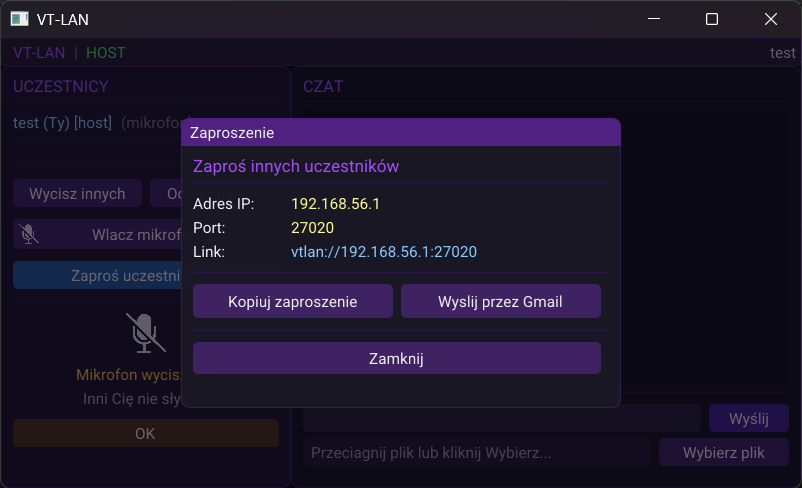
\includegraphics[width=0.70\textwidth]{figures/repo/invite.png}
    \caption{Ekran zaproszenia uczestników (praca własna)}
    \label{fig:repo_invite}
\end{figure}

\begin{itemize}
    \item \textbf{Kopiuj zaproszenie do schowka} -- kliknięcie przycisku
    kopiuje gotowe zaproszenie zawierające adres IP, port oraz link do pokoju.
    Skopiowaną treść należy wkleić (\textbf{Ctrl+V}) w wybranym komunikatorze
    lub wiadomości e-mail i przesłać zapraszanej osobie.
    \item \textbf{Zaproszenie przez Gmail} (\textit{opcjonalne}) --
    umożliwia wysłanie zaproszenia bezpośrednio z konta Gmail.
\end{itemize}

\begin{quote}
\textbf{Ważne:} Zaproszenie jest ważne wyłącznie w obrębie tej samej sieci
lokalnej. Zapraszany uczestnik musi być podłączony do \textbf{tej samej
sieci Wi-Fi lub LAN co host}.
\end{quote}

\subsection*{Pokój rozmów -- obsługa aplikacji}

Po dołączeniu do pokoju wyświetlany jest główny ekran aplikacji
(rysunek~\ref{fig:repo_chatroom}).

\begin{figure}[H]
    \centering
    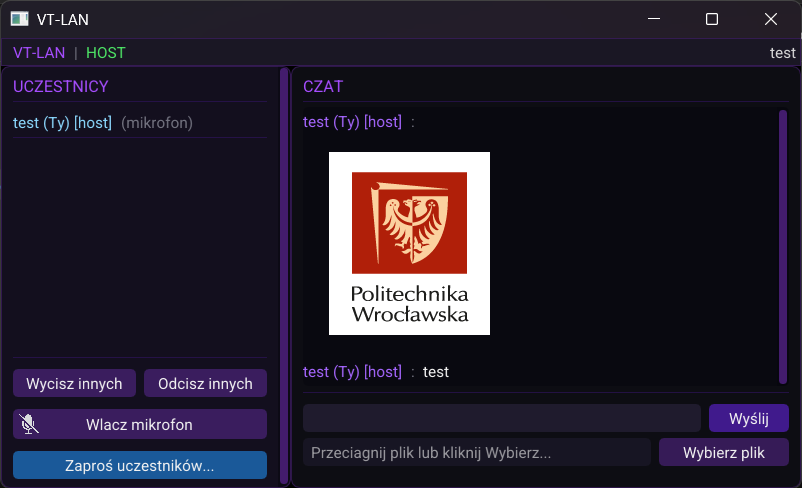
\includegraphics[width=0.90\textwidth]{figures/repo/chatroom.png}
    \caption{Główny ekran pokoju rozmów (praca własna)}
    \label{fig:repo_chatroom}
\end{figure}

\textbf{Lista uczestników.}
Po jednej ze stron ekranu widoczna jest lista wszystkich aktualnie
połączonych uczestników wraz z ich imionami i nazwiskami.

\textbf{Mikrofon -- wyciszanie i odciszanie.}
Przycisk z ikoną mikrofonu służy do wyciszania i odciszania mikrofonu.
Pierwsze kliknięcie wycisza mikrofon; ponowne kliknięcie odcisza.
Wyciszenie nie przerywa połączenia -- dźwięk od pozostałych uczestników
jest nadal odbierany.

\textbf{Wysyłanie plików.}
Aplikacja obsługuje dwa sposoby wysyłania plików:

\begin{enumerate}
    \item \textbf{Przeciągnij i upuść} (\textit{drag \& drop}) --
    należy otworzyć folder z plikiem, chwycić go i przeciągnąć na okno
    aplikacji, a następnie zwolnić przycisk myszy.
    \item \textbf{Wybór pliku z dysku} -- należy kliknąć ikonę wyboru pliku
    w interfejsie aplikacji, przejść do docelowego pliku i otworzyć go.
\end{enumerate}

Odebrane pliki zapisywane są automatycznie w folderze \texttt{received\_files/}
w katalogu aplikacji.

\subsection*{Wymagania systemowe i rozwiązywanie problemów}

Wymagania systemowe oraz szczegółowe procedury rozwiązywania typowych
problemów z uruchomieniem i połączeniem (m.in. konfiguracja reguł zapory
systemowej dla ruchu UDP na porcie aplikacji) zawarte są w pliku
\texttt{README.md} w repozytorium projektu. Dokument ten jest na bieżąco
aktualizowany i stanowi podstawowe źródło informacji dla użytkowników
aplikacji.

% ─────────────────────────────────────────────────────────────────────────────
\section{Dystrybucja i dalszy rozwój projektu}
\label{sec:distribution}
% ─────────────────────────────────────────────────────────────────────────────

Zgodnie z założeniami opisanymi we wstępie projektu, VT-LAN stanowi
darmową, open-source'ową alternatywę dla komercyjnych komunikatorów,
redukującą koszty infrastruktury i chroniącą prywatność użytkowników
poprzez działanie wyłącznie w sieci lokalnej. Po ukończeniu prac
implementacyjnych projekt został opublikowany publicznie w serwisie
GitHub pod adresem \url{https://github.com/Panogrodek/VT-LAN}
(rysunek~\ref{fig:github_repo}).

\begin{figure}[H]
    \centering
    % Wstaw zrzut ekranu strony repozytorium GitHub
    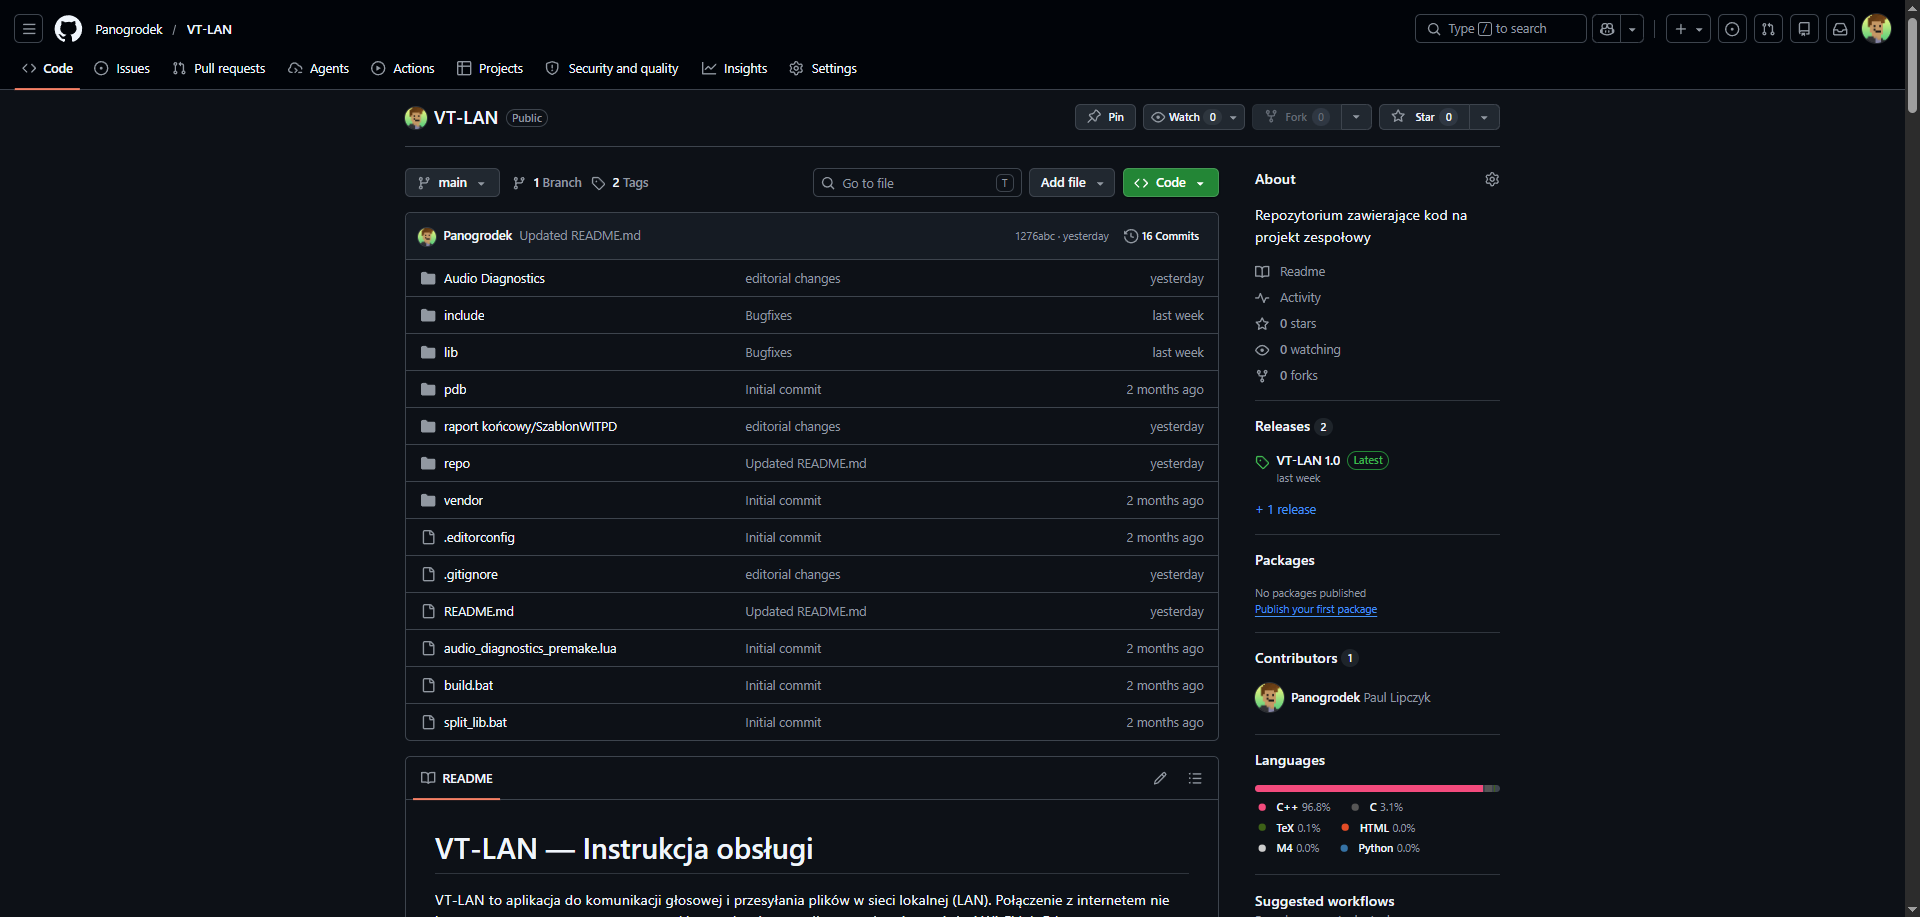
\includegraphics[width=0.95\textwidth]{figures/vtlan_github.png}
    \caption{Repozytorium projektu VT-LAN w serwisie GitHub (praca własna)}
    \label{fig:github_repo}
\end{figure}

Repozytorium zawiera kompletny kod źródłowy aplikacji, gotowe pliki
binarne w zakładce \textit{Releases} umożliwiające natychmiastowe
uruchomienie bez konieczności kompilacji, a także pełną instrukcję
obsługi w pliku \texttt{README.md}. Licencja open source oznacza,
że każdy zainteresowany użytkownik może pobrać, uruchomić i modyfikować
aplikację zgodnie z własnymi potrzebami.

Zrealizowany projekt potwierdza, że możliwe jest zbudowanie lekkiego,
bezpiecznego komunikatora głosowo-tekstowego działającego wyłącznie
w obrębie sieci lokalnej, bez udziału zewnętrznej infrastruktury.
Przeprowadzone testy (rozdział~\ref{ch:profilowanie_debugging})
potwierdziły spełnienie założeń dotyczących niskiego zużycia zasobów,
skuteczności mechanizmu VAD oraz poufności transmisji, a otwarty model
rozwoju stwarza warunki do dalszej rozbudowy aplikacji w kierunkach
opisanych w sekcji~\ref{sec:dalsza_rozbudowa_ui}.
